\section{The Large Hadron Collider}
In March 1984, the European Organization for Nuclear Research CERN) and the European Committee for Future Accelerators (ECFA) 
held a workshop in Lausanne entitled "Large Hadron Collider in the LEP Tunnel". 
This is history's first written mention of the Large Hadron Collider (LHC) and the topic under discussion 
was exactly how and where to build a new type of high-energy collider, capable of bringing hadrons
to collide rather than leptons.
The LHC would be housed in a tunnel which, at the time, was under excavation to host the Large Electron-Positron Collider (LEP) designed to collide leptons with center-of-mass-energies up to around 200 \GeV.
LEP was a circular collider with a circumference of 27 km and the tunnel hosting it was located roughly 100 meters underground on the border between France and Switzerland, at the outskirts of Geneva. 
The justification for building a machine like the LHC, was that once LEP got to maximum reach, a new and more powerful collider would be needed in its place in order to probe higher energies.
While collisions of electrons with positrons provided exceptionally clean and precise measurements due to them being point particles,
 their lightness prevent them from being accelerated to higher energies. Collisions of hadrons, however, would allow for center-of-mass energies two orders of magnitude higher than that of LEP. Therefore, after running a while at two times the W mass (160 \GeV) and reaching a maximum center-of-mass energy of 209 \GeV, LEP was dismantled in 2000 in order to make room for the LHC.
 
The Large Hadron Collider started up in September 2008 and, while having the same 27-kilometer radius as the LEP collider, is capable of accelerating protons up to a center-of-mass energy of around 14 TeV, 70 times that of LEP. The accelerator consists of two oppositely going proton beams, isolated from each other and under ultrahigh vacuum, which are accelerated up to speeds close to that of the speed of light through radio frequency (RF) cavities, before being brought to collide at four different interaction points along the ring.
These four collision points correspond to the location of the four LHC particle detectors; ATLAS, CMS, LHCb and ALICE.
While ATLAS and CMS are general-purpose detectors built in order to study a large range of different physics processes, 
LHCb and ALICE are built for dedicated purposes; LHCb for b-physics processes and ALICE for heavy ion collision.
A protons journey from gas to one of the LHC collision points is as follows: First, hydrogen nuclei are extracted from a small tank of compressed hydrogen gas and stripped of their electrons. The remaining protons are then
injected into the LINAC2, a linear accelerator responsible for increasing the proton energy to about 50 MeV through RF cavities that push charged particles forward by switching from positive to negative electric fields. LINAC2 additionally divides the constant stream of particles into equally spaced "bunches" by careful tuning of the frequency of the field switch.
The accelerated protons are then injected into the Proton Synchrotron Booster (PSB), where their energy is increased thirty folds more, to an energy of roughly 1.4 \GeV. The two final acceleration stages before the protons reach the LHC ring are the Proton Synchrotron and Super Proton Synchrotron, eventually leaving the protons with a total energy of 450 \GeV. The protons are now ready for the final stage of their travel and are injected into the two beam pipes of the LHC in oppositely going direction. They are injected in trains of 144 bunches each ( with an order of $10^{11}$ protons per bunch), where each bunch is roughly 7.5 meters apart (or 25 ns). There are some larger beam gaps present in each beam in order to give the beam dump and injection kickers sufficient time to reach full voltage, where the largest one, the beam abort gap,  is roughly 3 ms or 900 m long. The ring is filled with proton bunches until these are equally distributed throughout the two rings, a process taking roughly 4 minutes. This is called a "fill". Here, the protons are accelerated to their maximum energy of 6.5 TeV, a process taking roughly 20 minutes, through eight RF cavities. These RF cavities are also responsible of keeping the proton bunches tightly bunched, ensuring maximum luminosity at the four collision points. A complete sketch of the CERN accelerator complex is shown in Figure~\ref{fig:cms:LHC}.

\begin{figure}[h] 
    \centering
    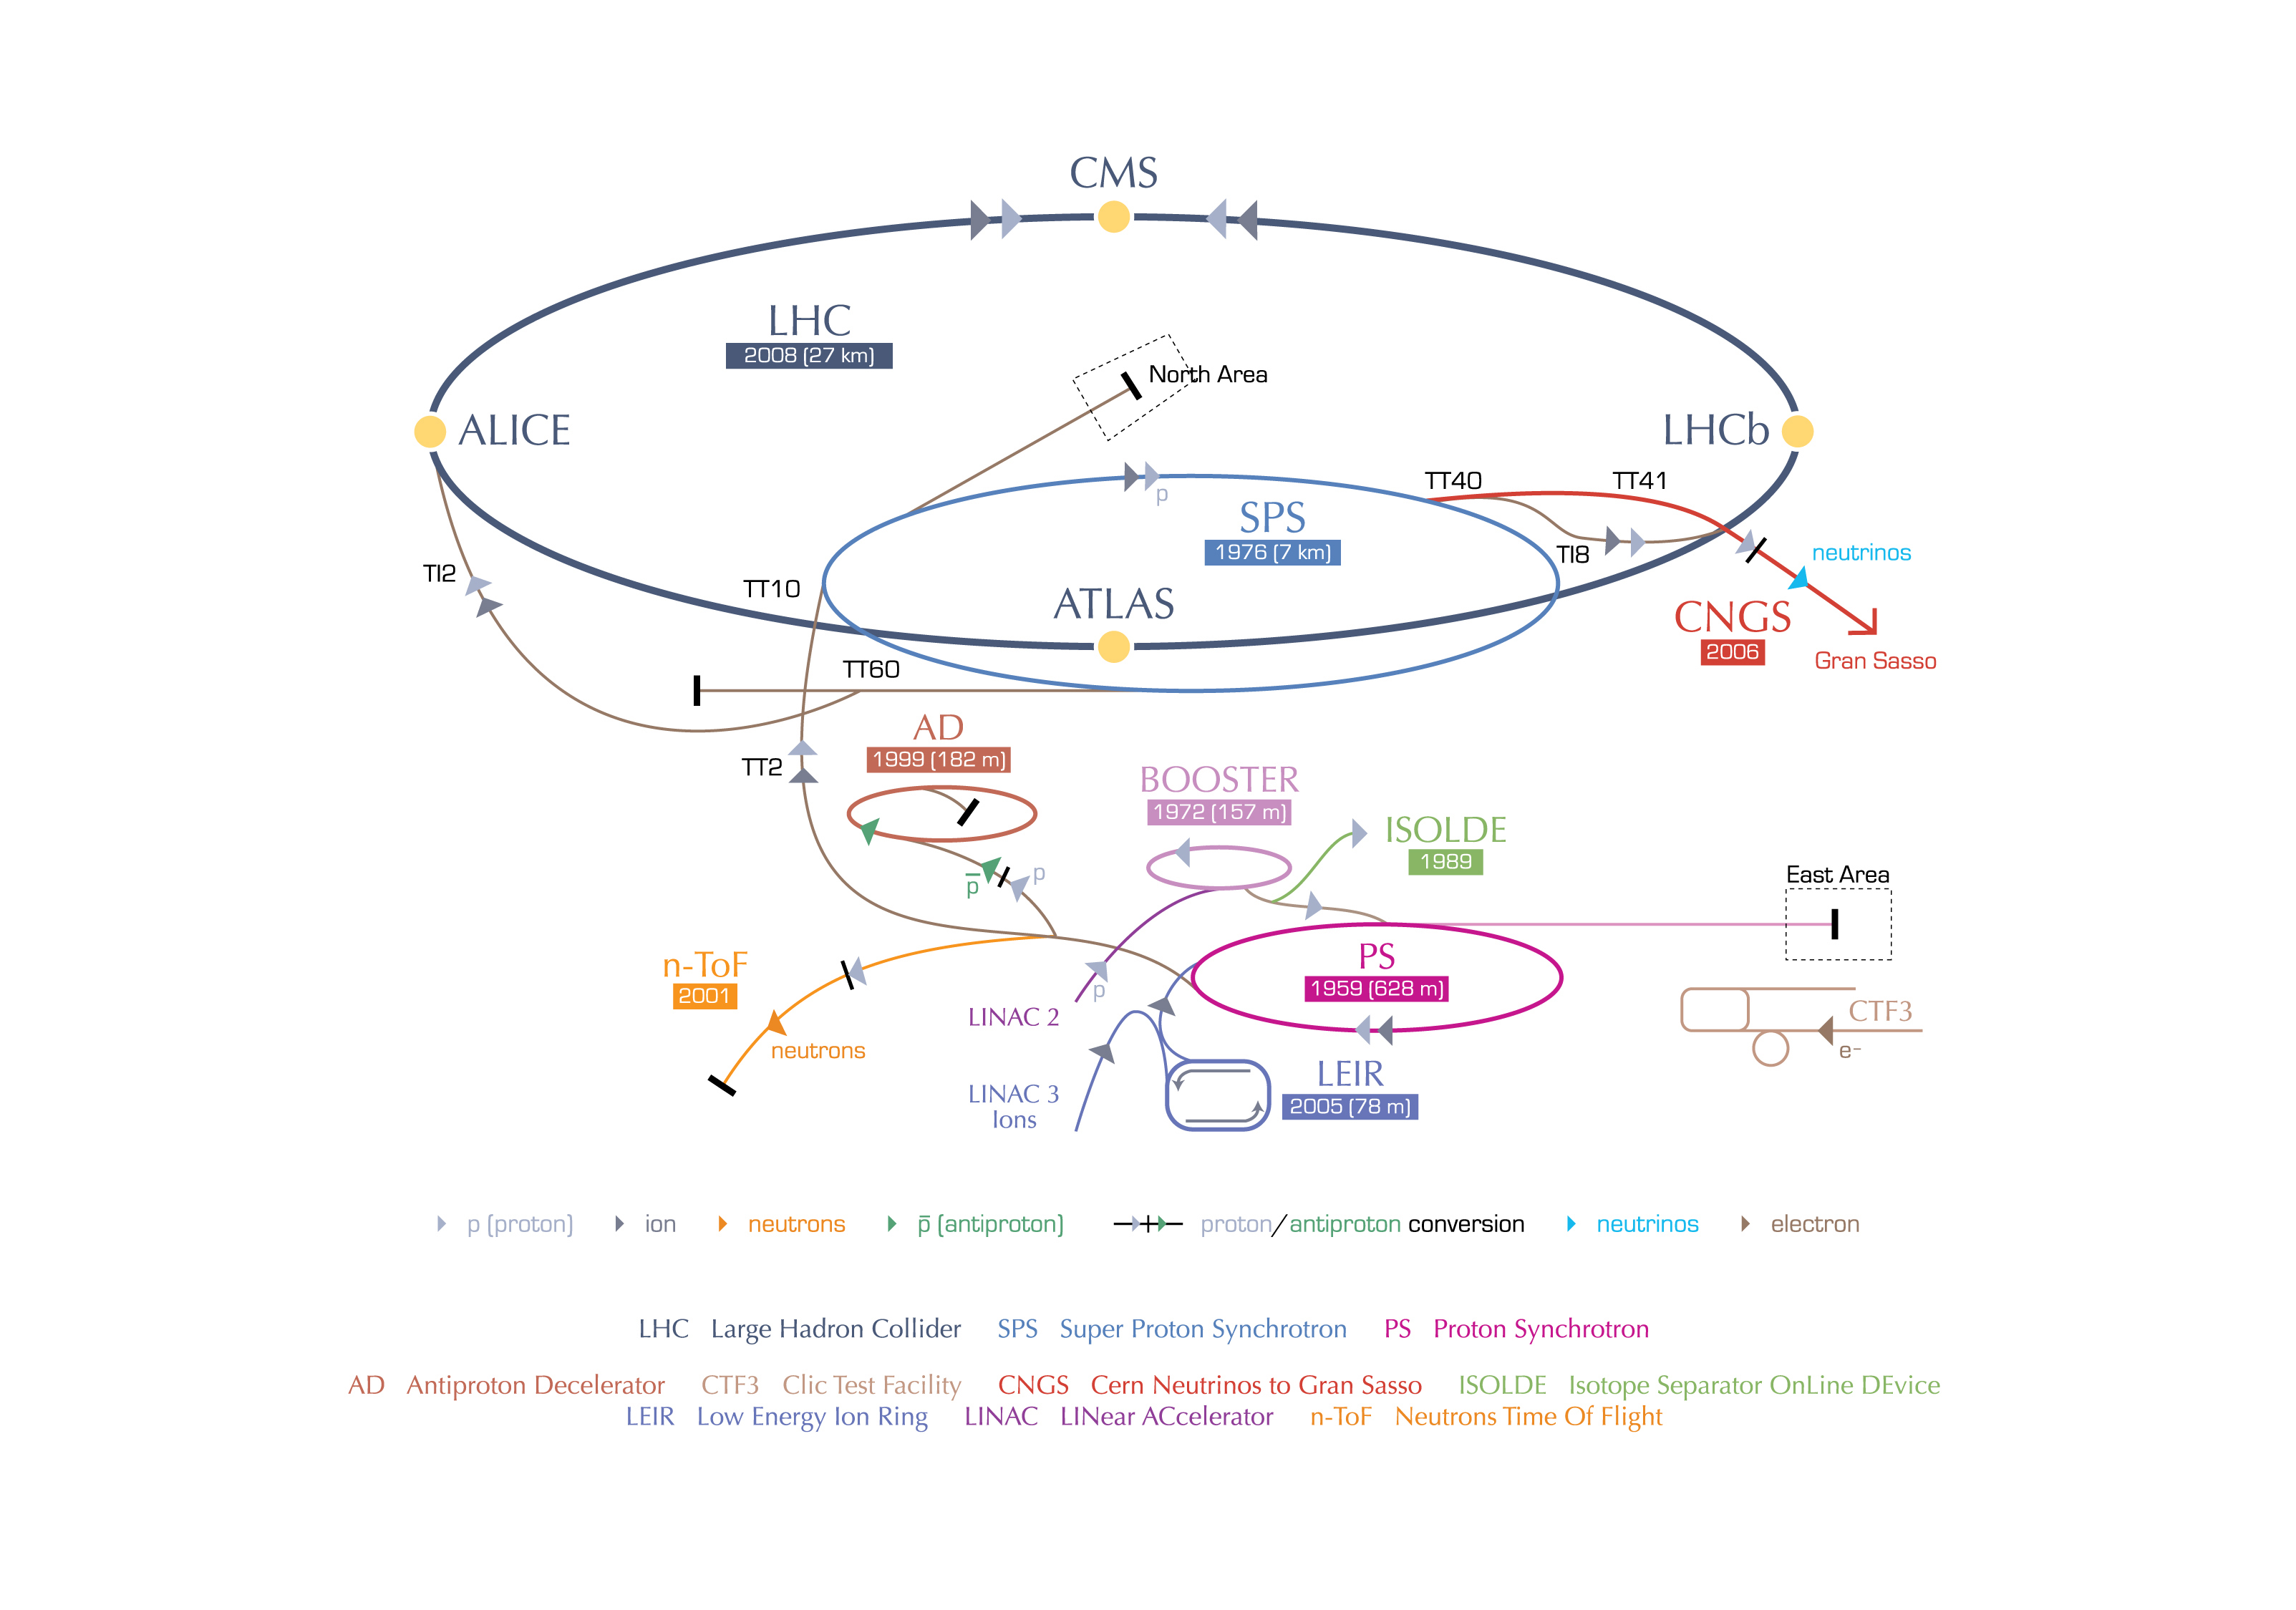
\includegraphics[width=1.0\textwidth]{figures/cms/LHC.jpg}
    \caption{The Large Hadron Collider accelerator complex. The four collision points along the ring correspond to the location of the LHC particle detectors CMS, LHCb, ATLAS and ALICE~\cite{LHC}.}
    \label{fig:cms:LHC}
\end{figure}

After the beams have reached their maximum energy and are stably circulating in the LHC ring, they are brought to collide. The goal of such a collision, which occurs every 25 nano seconds, is that some of the protons will undergo an inelastic collision, allowing the quark/gluon constituents of each proton to interact with one another and produce new and interesting particles.
The number of times such an interaction will take place inside a detector per area and time is quantified through the luminosity,$\mathcal L$, which is the proportionality factor between the number of observable events per second, and the cross section $\sigma$ of the process you are interested in
 
\begin{equation}
  \frac{dN_{events}}{dt} =\mathcal L \sigma .
\end{equation}

The cross section is the probability that an event (like one which would produce new and interesting particles) will occur and is measured in barns, where $1 \textrm{ barn} = 10^{-28} \textrm{ m}^2$. This proportionality factor should therefore be as high as possible. It depends only on parameters of the detector and can, in the case of LHC, be defined through the following accelerator quantities

\begin{equation}
  \mathcal L = \frac {N_b^2 n_b f_{rev} \gamma_r} {4 \pi \epsilon_n \beta *}F,
\end{equation}

where $N_b$ is the number of particles per bunch, $n_b$ is the number of bunches, $f_{rev}$ is their revolution frequency, $\gamma_r$ is the relativistic gamma factor,
$\epsilon_n$ is the transverse beam emittance (how confined the particles are in space and momentum), $\beta *$ is the beta function at the collision point (how narrow, or "squeezed", the beam is) and F is a reduction factor to account for a constellation where the beams do not collide heads-on but at slight crossing angles.
From this, it becomes clear that the main goal of the LHC is to; maximize the number of particles ($N_b$,$n_b$), their frequency ($f_rev$) and their energy ($\gamma_r$),
while at the same time ensuring the protons are packed together as tightly as possible (lower $\epsilon_n$ and $\beta *$).
Using the nominal values of the LHC, the peak luminosity is roughly $\mathcal L \sim 10^{34} \textrm{cm}^{-2} s^{-1}$. 


The peak luminosity of the LHC by the end of Run 2 in 2018 was grazing around $2.0 \cdot 10^{34} \textrm{cm}^{-2} s^{-1}$, corresponding to 2 times the nominal design luminosity.

To quantify the size and statistical power of a given LHC dataset, the integrated luminosity is used. This it the integral of the instantaneous luminosity over time and is defined as

\begin{equation}
  \mathcal L_{int} = \int \mathcal L dt.
\end{equation}

It is usually defined in units of inverse cross section, $\textrm{b}^{-1}$.


Despite the LHC starting up in 2008, there would be another year before data taking began.In March 2010, the LHC saw its first collision with a center-of-mass energy of 7 TeV, and continued running at this energy collecting around 5 inverse femtobarns of data by the end of 2011. In 2012, the energy was increased to 8 TeV and the LHC continued running until a planned long shutdown scheduled to begin in February 2013, collecting a total of $\sim 20 \textrm{ fb}^{-1}$ and discovering the Higgs boson. 
This marked the end of Run 1 and the beginning of a two-year maintenance project intended to prepare the LHC for running at a center-of-mass energy of 13 TeV; Run 2.

Run 2, and where this thesis begins, started in June 2015. With the accelerator now running at 90\% of its nominal energy, and with a peak luminosity between 1-2 times the design luminosity, the LHC managed to collect an impressive $\sim 160 \textrm{ fb}^{-1}$ at this energy until its planned shutdown at the end of 2018. Some key LHC accelerator parameters that were in use for the datasets analyzed in this thesis, are quoted in Table~\ref{tab:LHCparameters}

\begin{table}[]
\begin{tabular}{| l | lllll |}
\hline
Parameter               & Units                                      & Nominal & 2015 & 2016 & 2017     \\
\hline
Energy                  & {[}TeV{]}                                  & 7.0     & 6.5  & 6.5  & 6.5      \\
Bunch spacing           & {[}ns{]}                                   & 25      & 25   & 25   & 25       \\
Bunch intensity         & $\times10^{11}${[}protons/bunch{]}         & 1.15    & 1.15 & 1.15 & 1.2-1.45 \\
Bunches per train       &                                            & 144     & 144  & 96   & 144      \\
Total number of bunches &                                            & 2808    & 2244 & 2220 & 2556     \\
$\beta*$                & {[}cm{]}                                   & 55      & 80   & 40   & 27/25    \\
Peak luminosity         & $\times 10^{34} [\textrm{cm}^{-2} s^{-1}]$ & 1.0     & 0.5  & 1.4  & 2.0      \\
Integrated luminosity   &                                            &         & 4.2  & 39.7 & 50.2     \\
\hline
\end{tabular}
\caption{Some key LHC detector parameters achieved during the first years of 13 TeV data taking}
\label{tab:LHCparameters}
%https://indico.cern.ch/event/663598/contributions/2782540/,https://indico.cern.ch/event/580313/contributions/2359285/attachments/1396590/2135891/Operation_in_2016_v1_1.pdf, http://iopscience.iop.org/article/10.1088/1748-0221/3/08/S08001/pdf
\end{table}


\section{The CMS detector}

The Compact Muon Solenoid (CMS) detector is true to its name; with a diameter of 15 meters and a weight of 14000 tons, it is 60 \% smaller but two times heavier than its general purpose counterpart, the ATLAS detector.
Its large weight is due to the CMS housing the worlds largest and most powerful solenoid: A superconducting niobium titanium coil circulating 18500 Amps and capable of generating a magnetic field of 3.8 Tesla. Together with its corresponding iron return yoke, responsible for reflecting the escaping magnetic flux, it accounts for 90\% of the total detector weight.
The CMS detector is cylindrically symmetric and organized in the following way: closest to the beam pipe and at a radius of about 3 cm, the inner tracking system begins. It consists of an inner silicon pixel detector and an outer silicon strip tracker, stretching out to a radius of roughly 1.2 meters. Following the tracker are two calorimeter layers: the electromagnetic calorimeter (ECAL) consisting of lead tungstate scintillating crystals and responsible for measuring the energy of electromagnetically interacting particles, followed by the hermetic hadronic calorimeter (HCAL) measuring the energy of hadrons.
Contrary to "standard" configurations for general purpose detectors, the CMS calorimeters are located inside the superconducting solenoid. This allows the detector to be rather compact, by reducing the necessary radius of the calorimeters, and additionally for the magnet to be strong enough (the magnetic field strength depends on the coil radius) to allow muon detectors to be located within the magnetic field so their momentum can be measured.
The muon detectors are alternated with three layers of steel return yoke responsible for containing and reflecting the magnetic field and which only allows muons and weakly interacting particles to pass. A schematic overview of the CMS detector is shown in Figure~\ref{fig:cms:CMS}. In the following, the different sub-detectors will be described in detail.

\begin{figure}[h] 
    \centering
    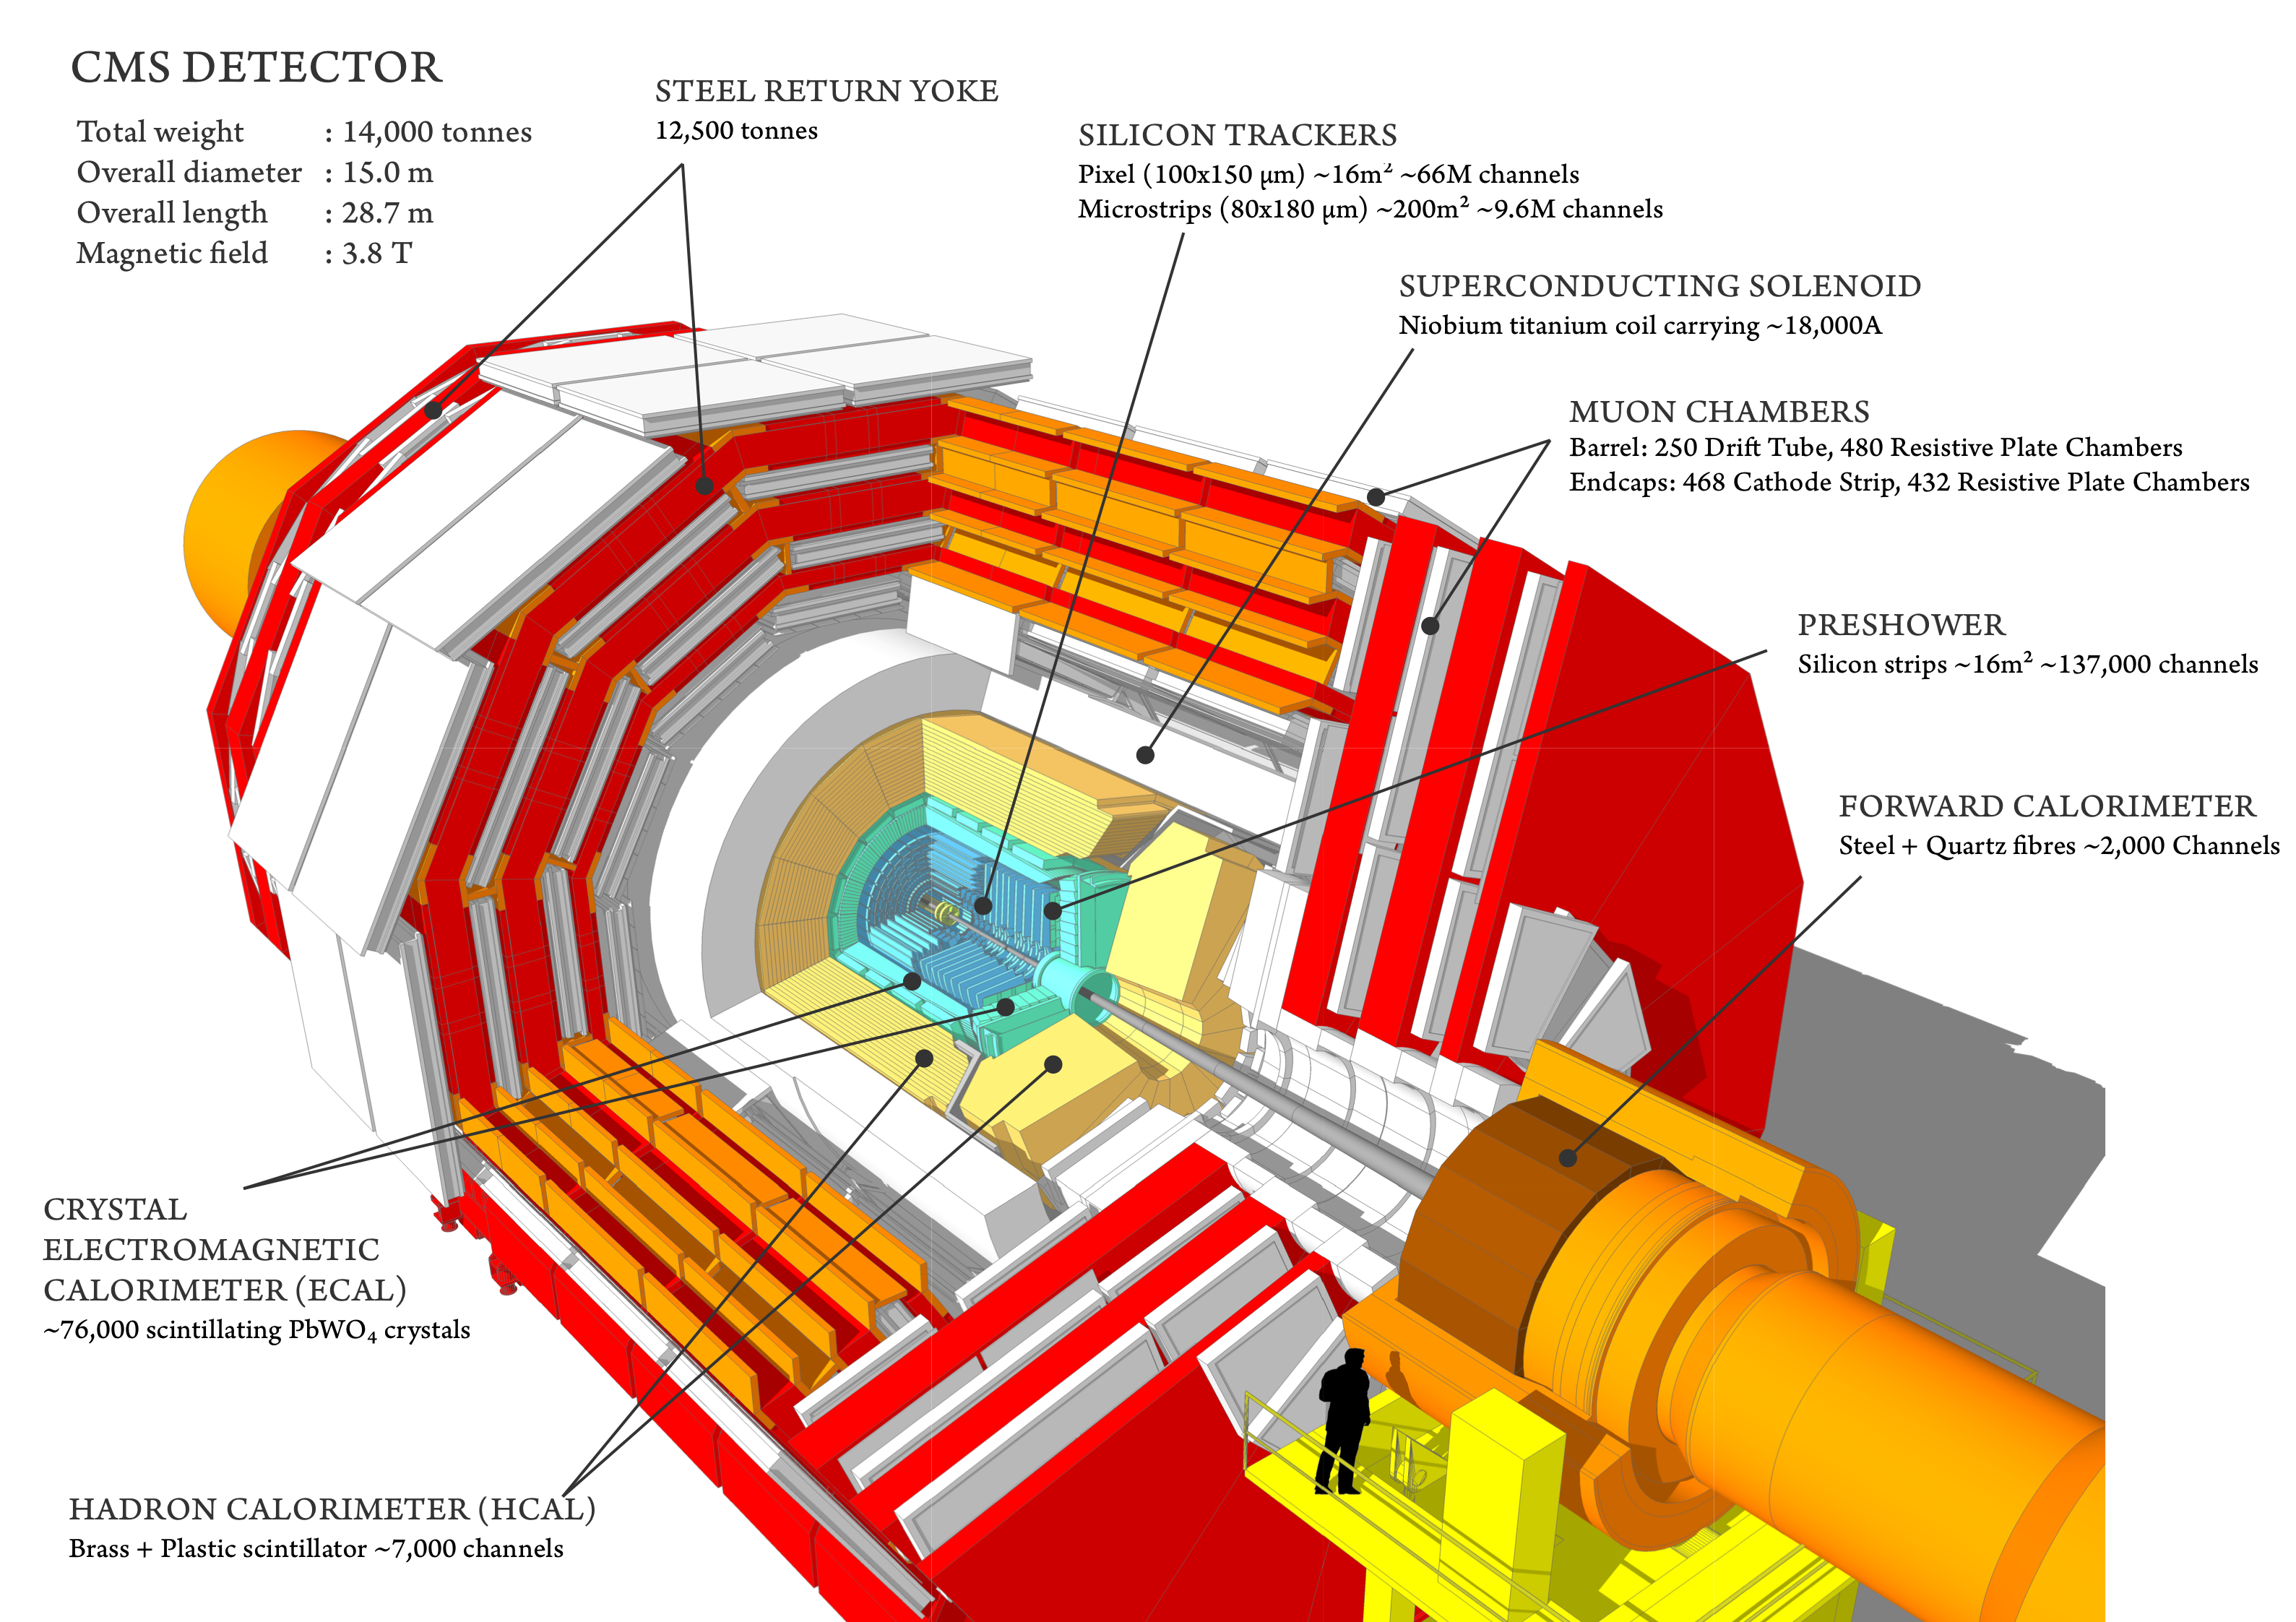
\includegraphics[width=1.0\textwidth]{figures/cms/CMS.png}
    \caption{The CMS detector and its subsystems: The silicon tracker, electromagnetic and hadron calorimeters, the superconducting solenoid and the muon chambers inter-layered with the steel return yoke~\cite{CMS}.}
    \label{fig:cms:CMS}
\end{figure}

\subsection{Coordinate system}
To describe locations within the CMS detector, a Euclidian space coordinate system is used. Here, the positive z axis points along the beam pipe towards the west, the positive x axis points towards the center of the LHC ring, and the positive y axis upw towards the earths surface. Due to the cylindrical symmetry of the detector, polar coordinates are more convenient and most frequently encountered. In this scheme, the azimuthal angle $\phi$ is measured in the xy-plane, where $\phi=0$ correspond to the positive x axis and $\phi=\pi/2$ correspond to the positive y axis. The polar angle $\theta$ is measured with respect to the z axis, $\theta=0$ aligning with the positive and $\theta=\pi$ with the negative z axis.
To define a particles angle with respect to the beam line, the pseudorapidity $\eta = -\ln{}\textrm{tan}(\theta/2)$ is preferred over $\theta$. This is due to the fact that particle production is approximately constant as a function of pseudorapidity and, more importantly, because differences in pseudorapidity are Lorentz invariant under boosts along the z-axis when assuming massless particles.
To measure angular difference between particles in the detector, the variable $\textrm{R}=\sqrt{\eta^2+\phi^2}$ is used, again Lorentz invariant under longitudinal boosts. A summary of the CMS coordinate system together with some example values are shown in Figure~\ref{fig:cms:coordinates}.


\begin{figure}[h] 
    \centering
    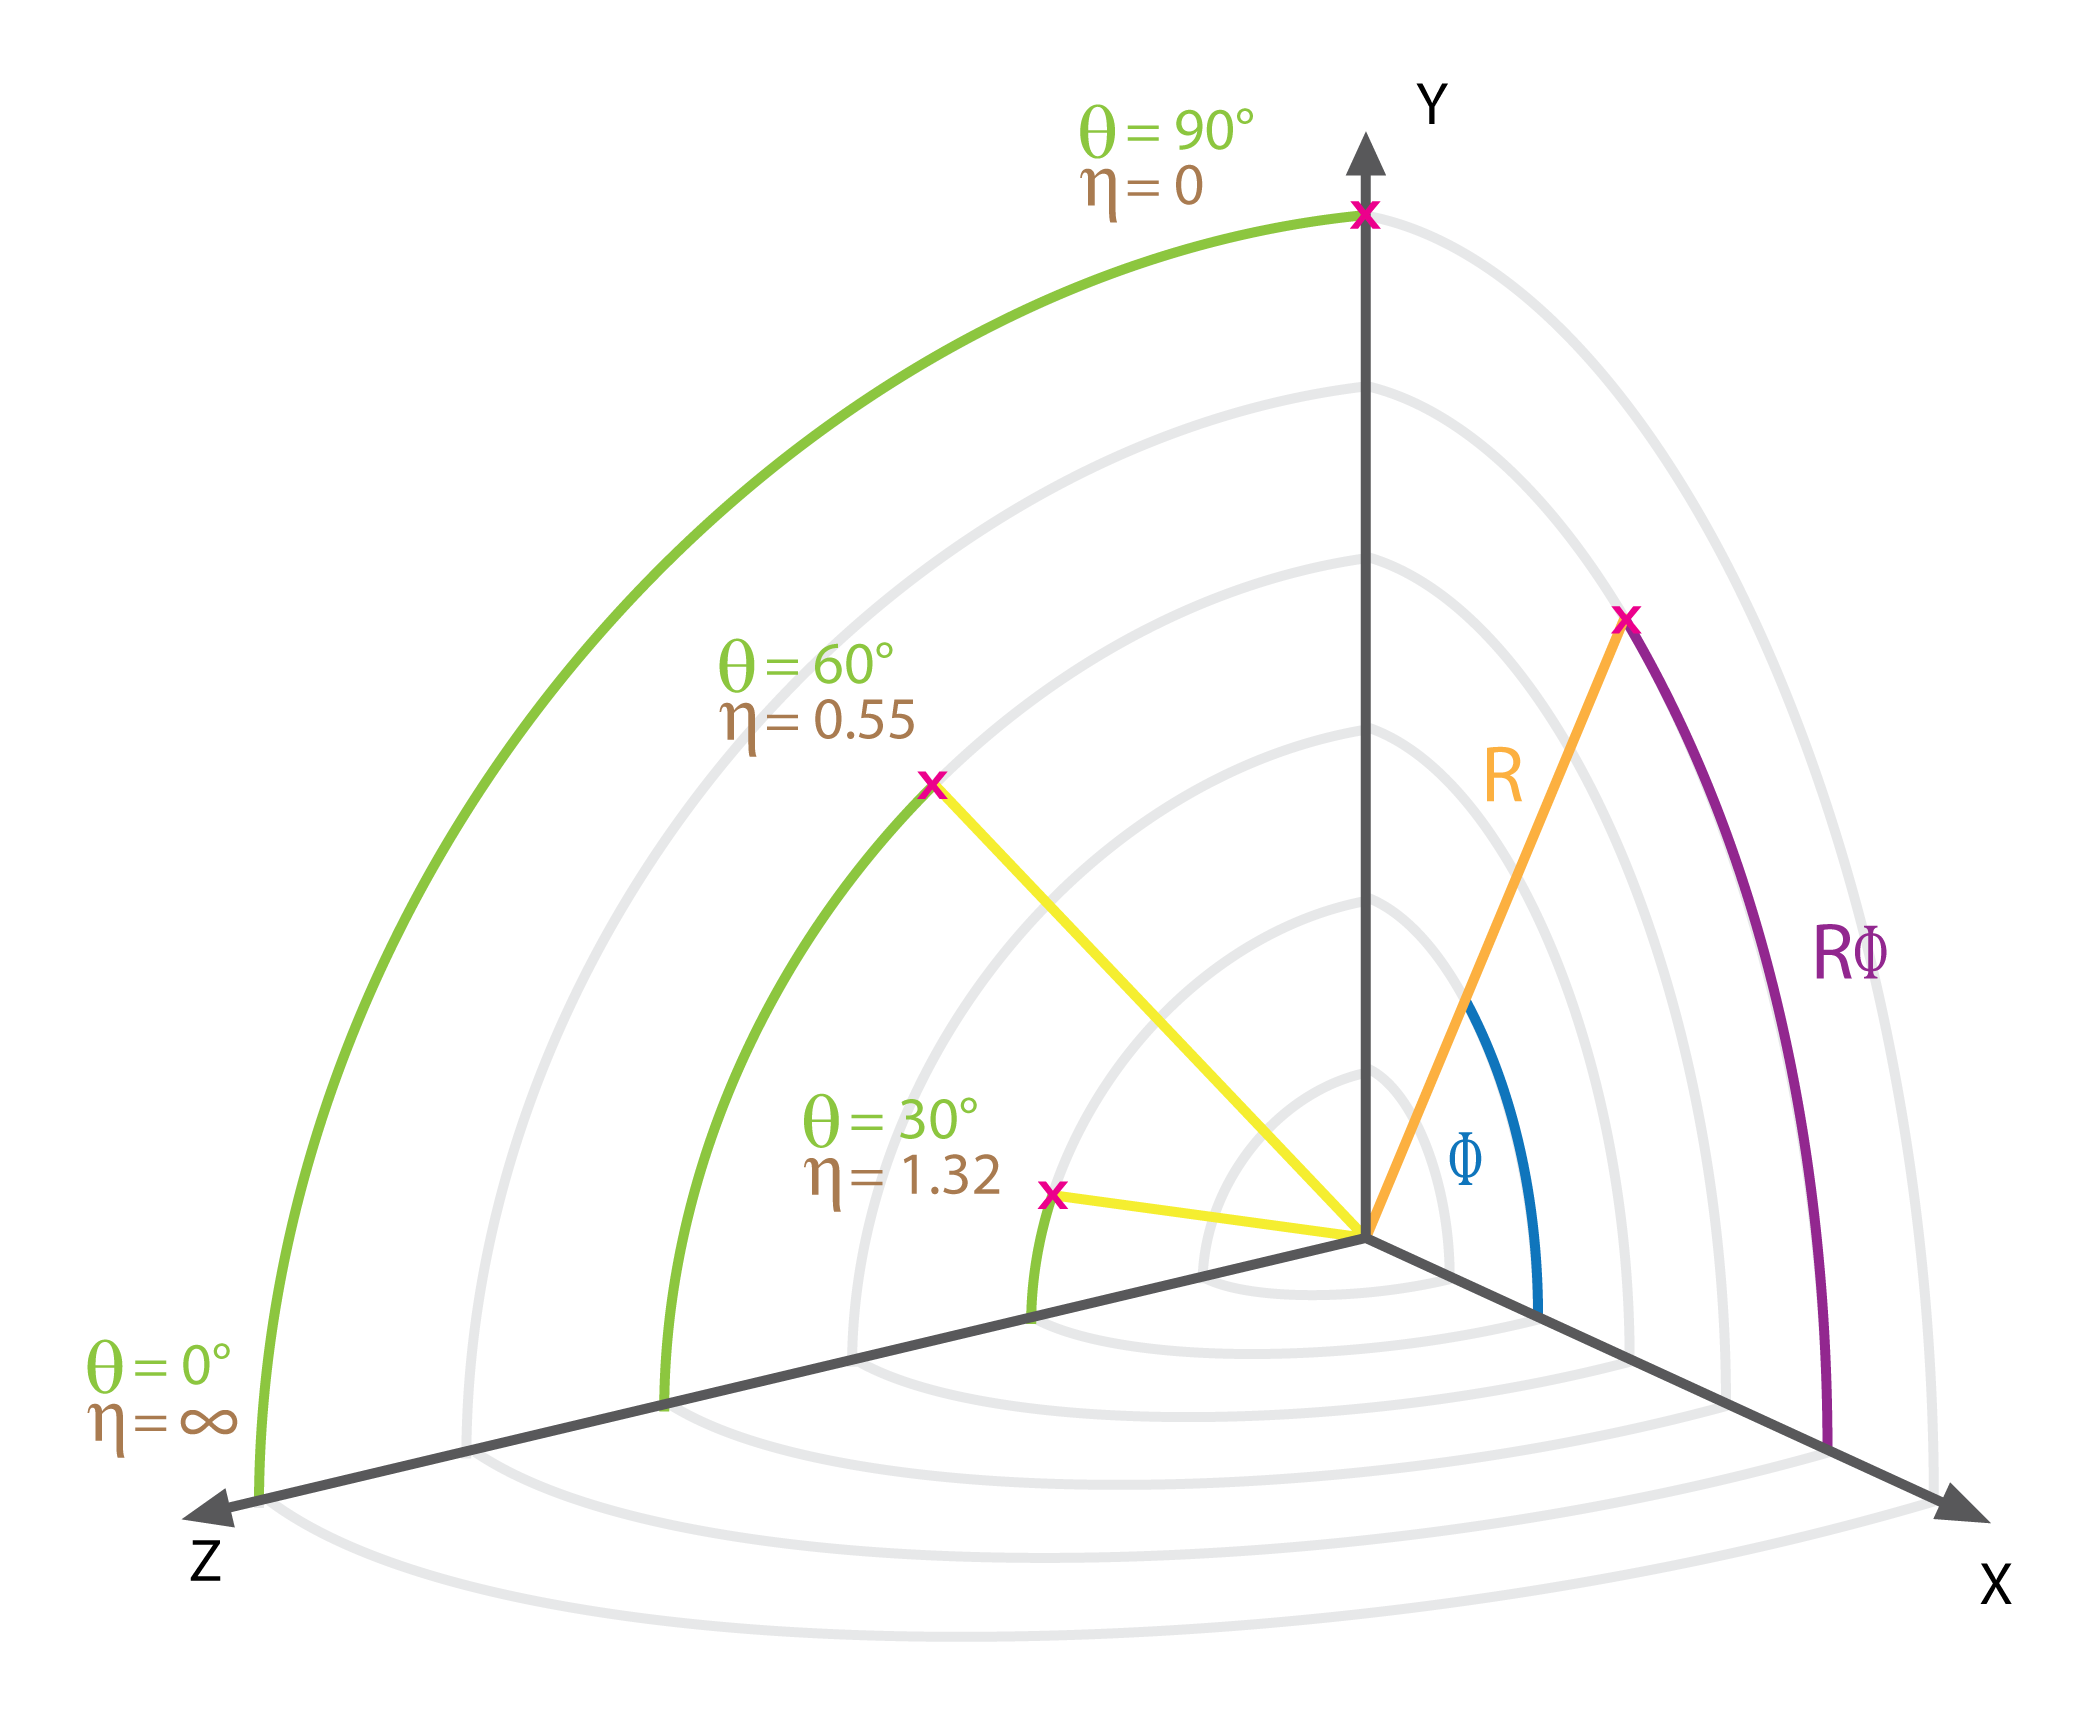
\includegraphics[width=0.45\textwidth]{figures/cms/img_cms_coordinates.png}
    \caption{The CMS coordinate system~\cite{Lenzi:2013xpa}}
    \label{fig:cms:coordinates}
\end{figure}


\subsection{Tracking detectors}
The CMS tracker is responsible for accurately reconstructing the momentum of charged particles and consists of two sub-detectors. Closest to the interaction point, and where the particle intensity is the highest, the silicon pixel detector is located. Upgraded in 2017, from the so-called Phase-0 to the Phase-1 layout, it is structured in four cylindrical barrel layers at radii 2.9, 6.8, 10.9 and 16.0 \cm (the barrel pixel) and three disks in each of the forward regions placed at a distance from the nominal interaction point of 29.1, 39.6 and 51.6 \cm (the forward pixel). A sketch of the current Phase-I pixel detector compared to the Phase-0 detector is shown in Figure~\ref{fig:cms:pixel}. The sensors located closest to the beam pipe are subject to hit intensities of $\mathcal{O}( \textrm{MHz}/\textrm{mm}^2 )$ which puts strict constraints on the maximum sensor size in order to minimize occupancy in the detector. The pixel sensors are 100 \micron x 150 \micron with a thickness of 285 \micron, and when counting both barrel and pixel sensors, sum up to a total of 79 million. The pixel sensors are mounted on detector modules with 16 read-out chips each, where the type of read-out chip depends on how close the module is to the beam pipe: the inner layer uses read-out chips with a rate capability of 600 MHz/$\cm^2$ while for the outer layers, read-out chips with a rate capability of up to 200 MHz/$\textrm{cm}^2$ are sufficient.

\begin{figure}[h] 
    \centering  
    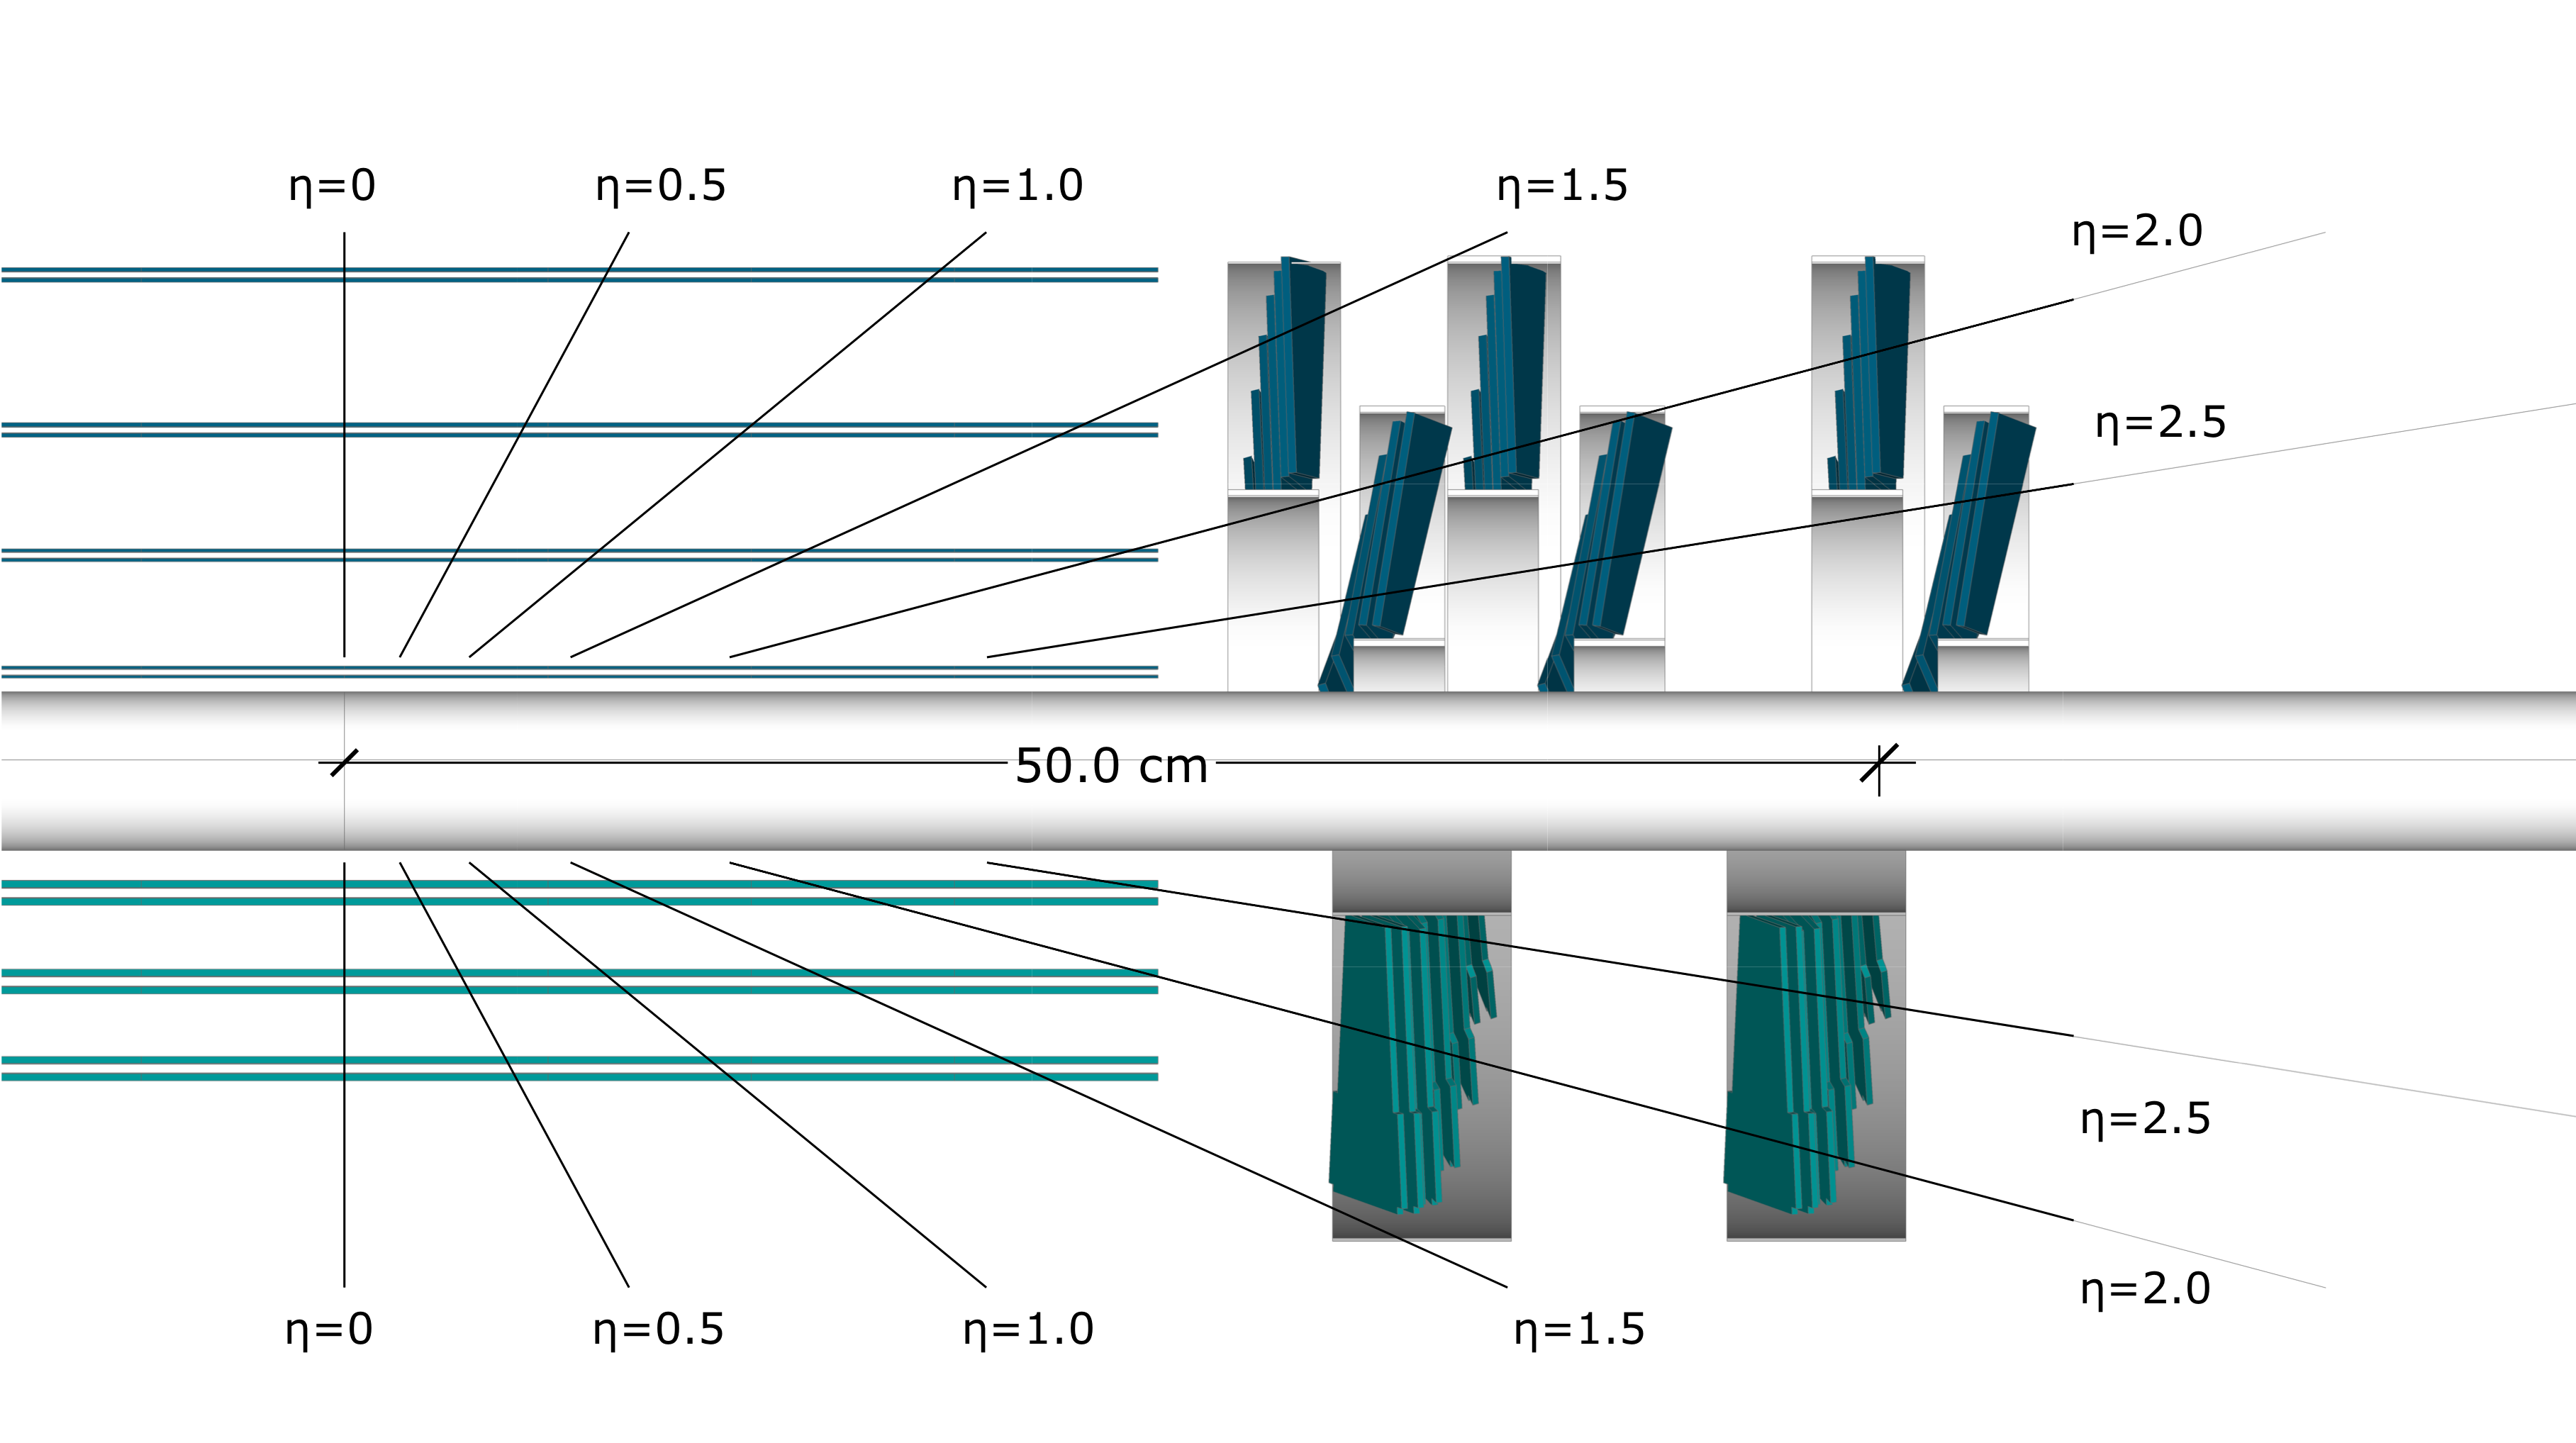
\includegraphics[height=4cm,keepaspectratio]{figures/cms/20120828_01_pixel_phase1_largesharp.png}
    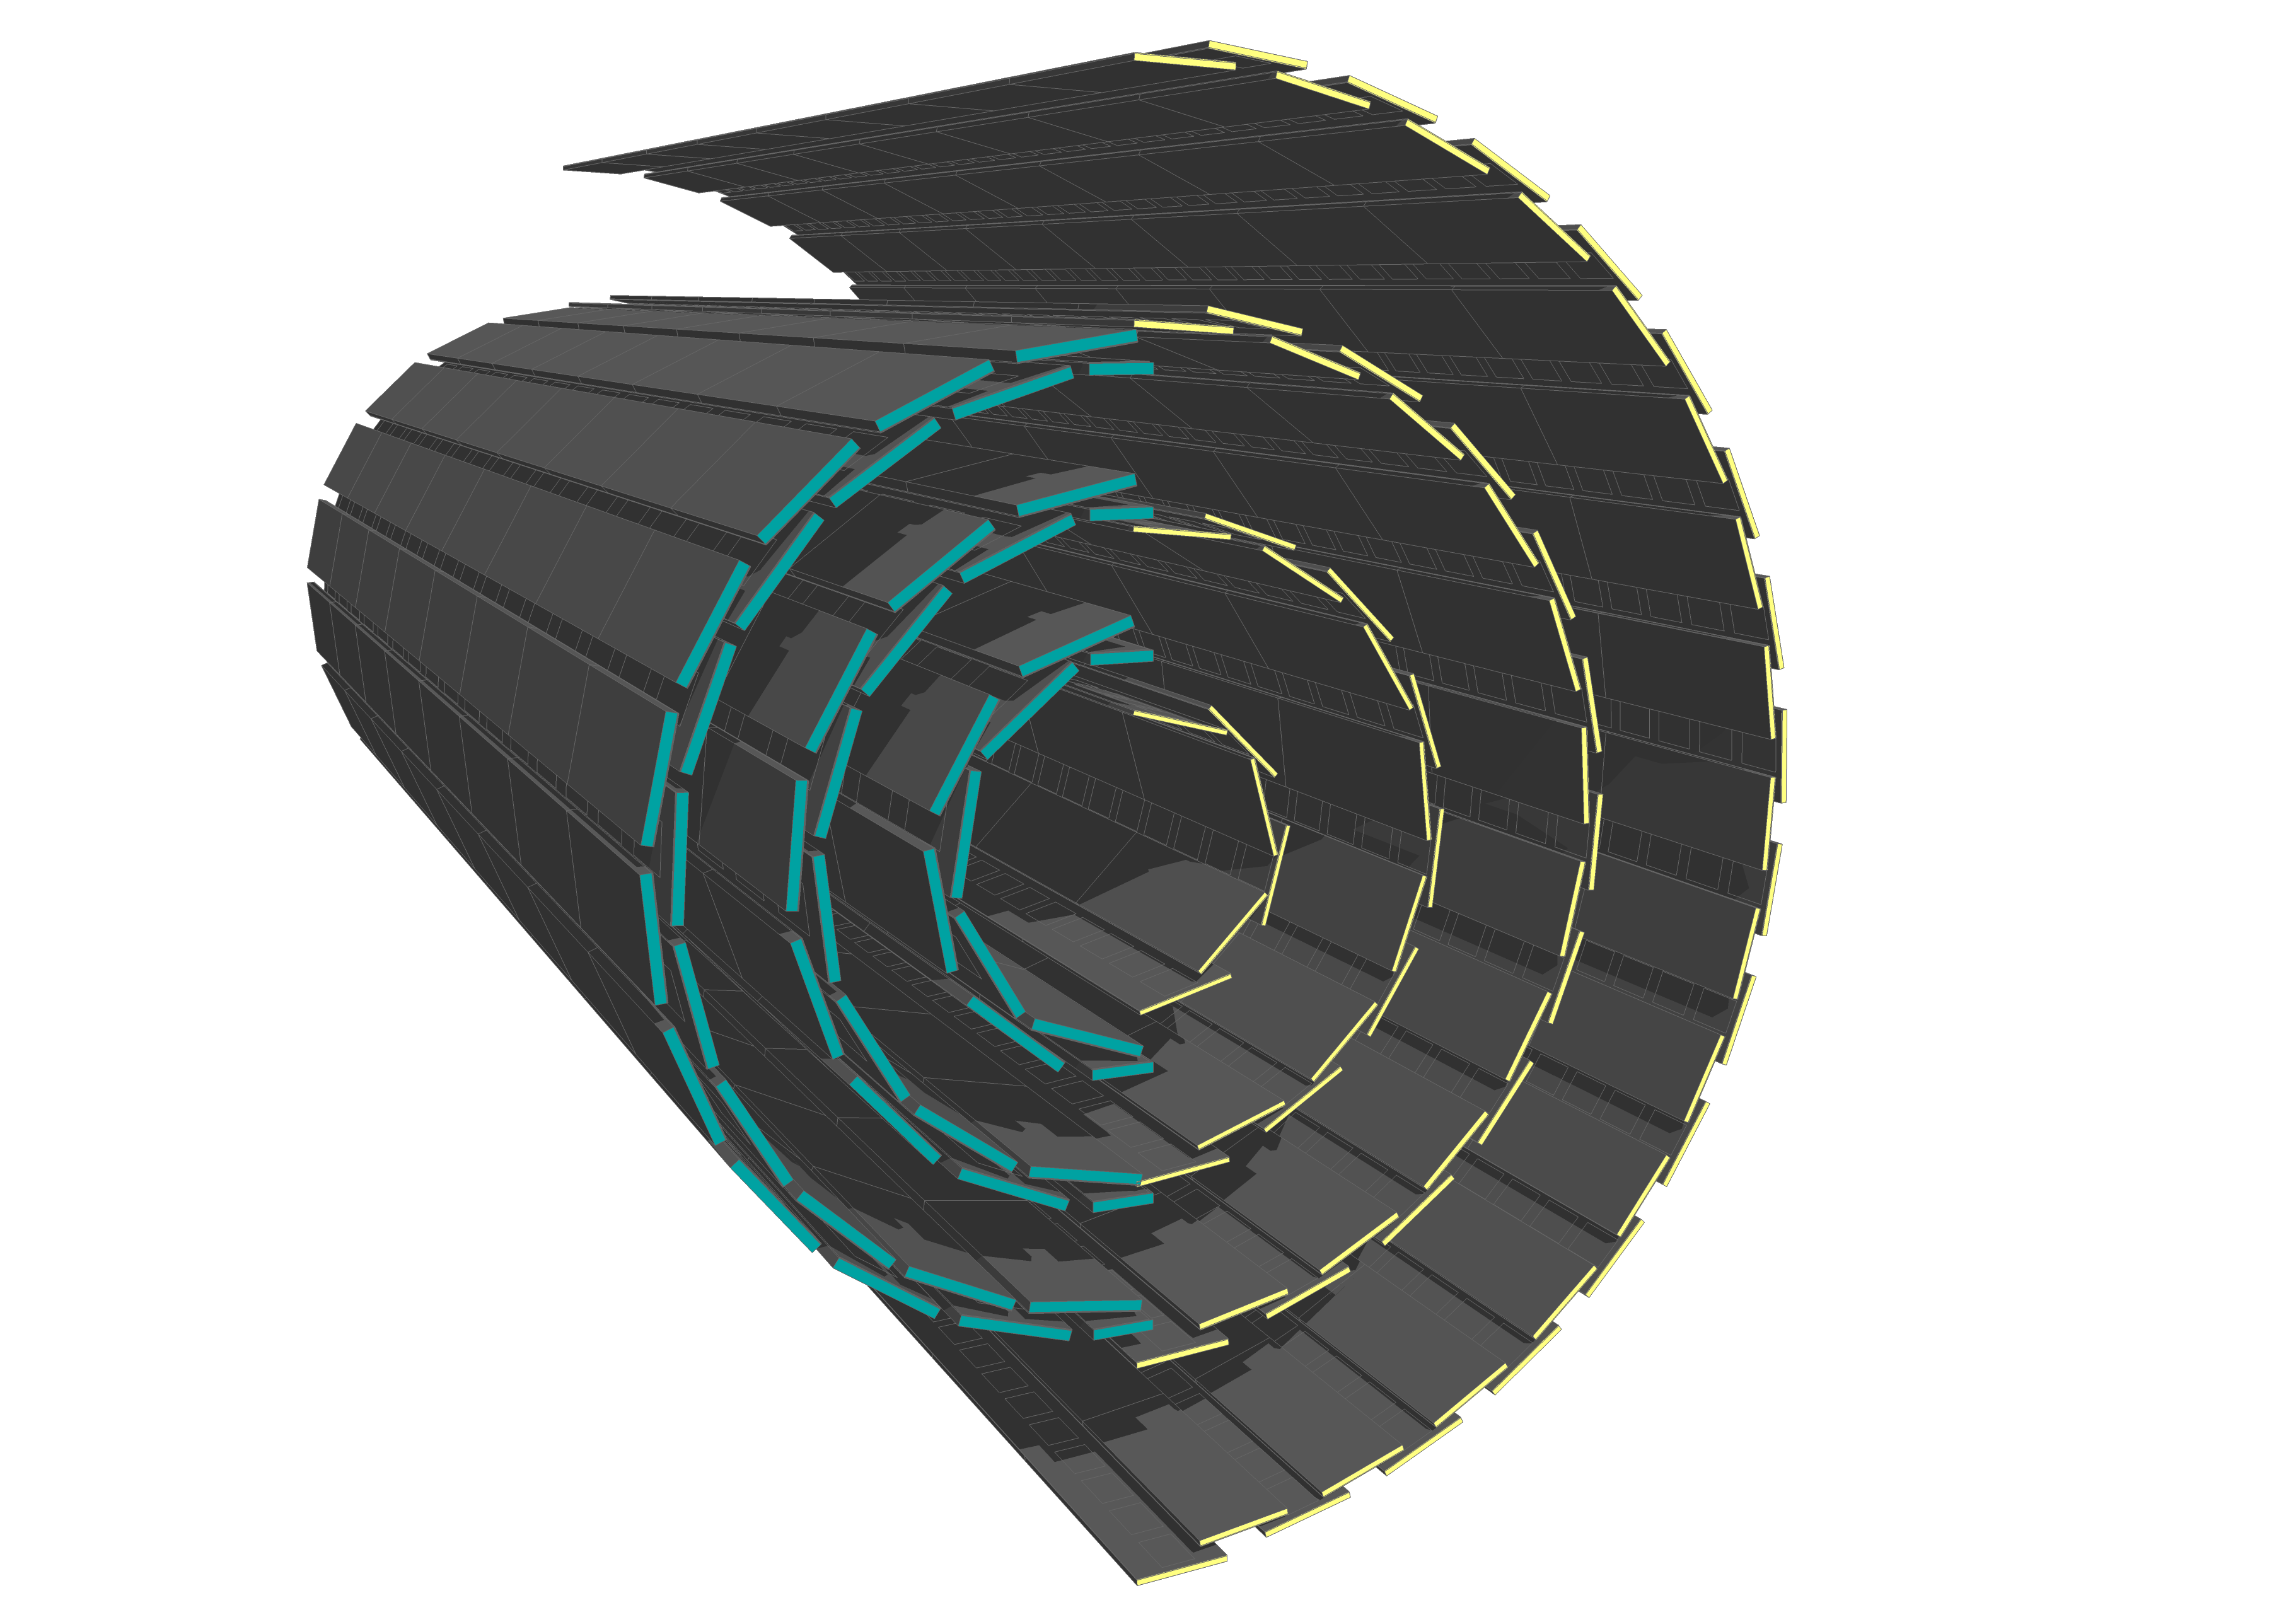
\includegraphics[height=4cm,keepaspectratio]{figures/cms/20120827_01_pixel_phase1_04.png}
    \caption{Left: The forward pixel detector layout before (bottom) and after (top) the Phase-I upgrade. Right: The barrel pixel detector before (left) and after (right) the Phase-I upgrade~\cite{Dominguez:1481838}.}
    \label{fig:cms:pixel}
\end{figure}

As the hit intensity reduces as you go further away from the beam pipe, the pixel sensors are replaced by silicon strip sensors, making up the second of the two tracker sub-systems, the silicon strip tracker. There are ten strip layers in total, stretching out to a radius of roughly 130 cm. These are divided into four sections: The inner barrel (TIB) with four strip layers, the two inner endcaps (TID) consisting of three disks each, the outer barrel (TOB) consisting of 6 cylindrical layers and the two endcaps (TEC) with 9 strip layers each. A schematic overview of the strip tracker layout is shown in Figure~\ref{fig:cms:tracker}.
The strips in the TIB and TID are 10 cm long, with a width of 80 \micron and a thickness of 320 \micron. The TOB and TEC sections consist of slightly larger strips of 25 \cm x 180 \micron and a thickness of 500 \micron. The strip tracker has a total of 10 million detector strips and covers an area of $\sim 200 \textrm{ m}^2$.
To prolong the silicon detector lifetime, the entire tracker (pixel and strip) is kept at a temperature of \SI{-20}{\celsius} through a liquid cooling system.
The tracker has a coverage up to $|\eta|<2.6$ and a resolution of roughly $\sigma / \PT \approx 1.5 \times 10^{-5} \PT \oplus 0.005$.

\begin{figure}[h] 
    \centering
    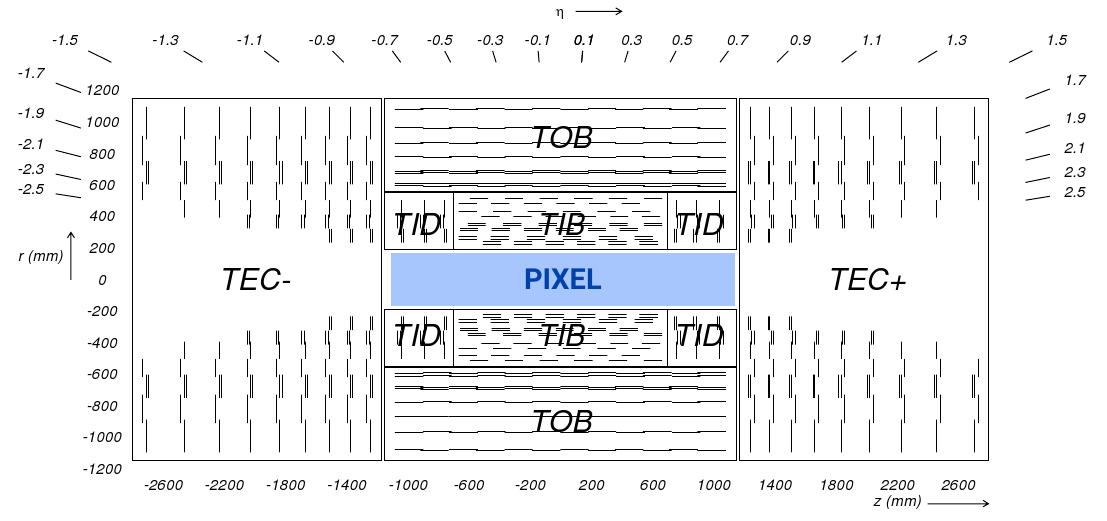
\includegraphics[width=1.0\textwidth]{figures/cms/fig_cmstracker.png}
    \caption{Schematic of the CMS silicon strip tracker and its four subsections: The inner barrel (TIB), inner endcaps (TID), the outer barrel (TOB) and the two endcaps (TEC)~\cite{Chatrchyan:2008aa}.}
    \label{fig:cms:tracker}
\end{figure}

\subsection{Electromagnetic calorimeter}
Following the tracking detectors is the electromagnetic crystal calorimeter (ECAL). Consisting of 75 848 laterally segmented scintillating lead tungstate ($\textrm{PbWO}_4$) crystals, it was designed to have the highest possible photon energy and position resolution in order to resolve a Higgs boson decaying into two photons, the cleanest of the Higgs discovery channels. 
With a goal of a photon/electron energy resolution of 0.5\% above 100 \GeV, the choice of detector material for the ECAL has been its most crucial design feature. 
In order to withstand the high doses of radiation and the high magnetic field present within the detector, while at the same time generating well-defined signal responses within the 25 nanoseconds between particle collisions, an extremely dense and transparent material capable of producing fast and clean photon bursts when hit, is required. 
The choice eventually fell on  metal-heavy lead tungstate crystals, each taking roughly two days to artificially grow (and a total of about ten years to grow all of them). With a density of $\delta=8.28 \textrm{ g}/\textrm{ cm}^3$ (slightly higher than for stainless steel), the crystals are compact enough to yield excellent performance without taking up too much volume, allowing the ECAL to sit within the CMS superconducting solenoid. The homogeneous medium allows for a better energy resolution as it minimizes sampling fluctuation effects and it additionally contains enough oxygen in crystalline form to make it highly transparent to their entire scintillation
emission spectrum. With an extremely short radiation length and small Moliére radius ($\textrm{X}_0=0.85$ \cm, $$\textrm{R}_M=2.19$$ \cm), the required homogeneity, granularity and compactness is obtained while at the same time emitting 80\% of generated light within the 25 ns timeframe required. The largest drawbacks with  a lead tungstate detector is the low light yield (100 $\gamma$ per MeV), requiring dedicated avalanche photodiodes to increase the gain, as well as a light yield which strongly depends on the temperature. The detector response to an
incident electron changes by 3.8 $\pm$ 0.4 \% per degree Celsius which requires the ECAL temperature to be kept stable around 18 \SI{18 \pm 0.05}{\degreeCelsius}, obtained through an intricate water cooling system.
The ECAL is completely hermetic and sorted into a barrel part (EB), covering pseudorapidities up to $|\eta|<1.48$, and two endcap parts (EE) extending the total coverage to $|\eta|<3.0$ in order to match the tracker coverage of $|\eta|<2.5$. In order to improve the $\gamma/\pi_0$ separation power, a pre-shower detector (ES) using lead absorbers and silicon sensors covers the forward region between $1.65<|\eta|<2.6$.
The  crystals in the barrel are organized into supermodules, each consisting of about 1700 crystals, while the endcap is divided into to half disks consisting of 3662 crystals each (so-called "Dees").
Each $\textrm{PbWO}_4$ crystal weighs around 1.5 kilogram and has a slightly tapered shape with a front face of 2.2 x 2.2 $\cm^2$ in the barrel and 2.86 x 2.86 $\cm^2$ in the endcaps. The crystals are 2.3 and 2.2 \cm long in the barrel and endcaps, respectively. The total volume of the calorimeter including barrel and endcaps is 11 $\textrm{m}^2$ and weighs a total of 92 tons.
The ECAL detector layout is illustrated in Figure~\ref{fig:cms:ecal}.


\begin{figure}[h] 
    \centering
    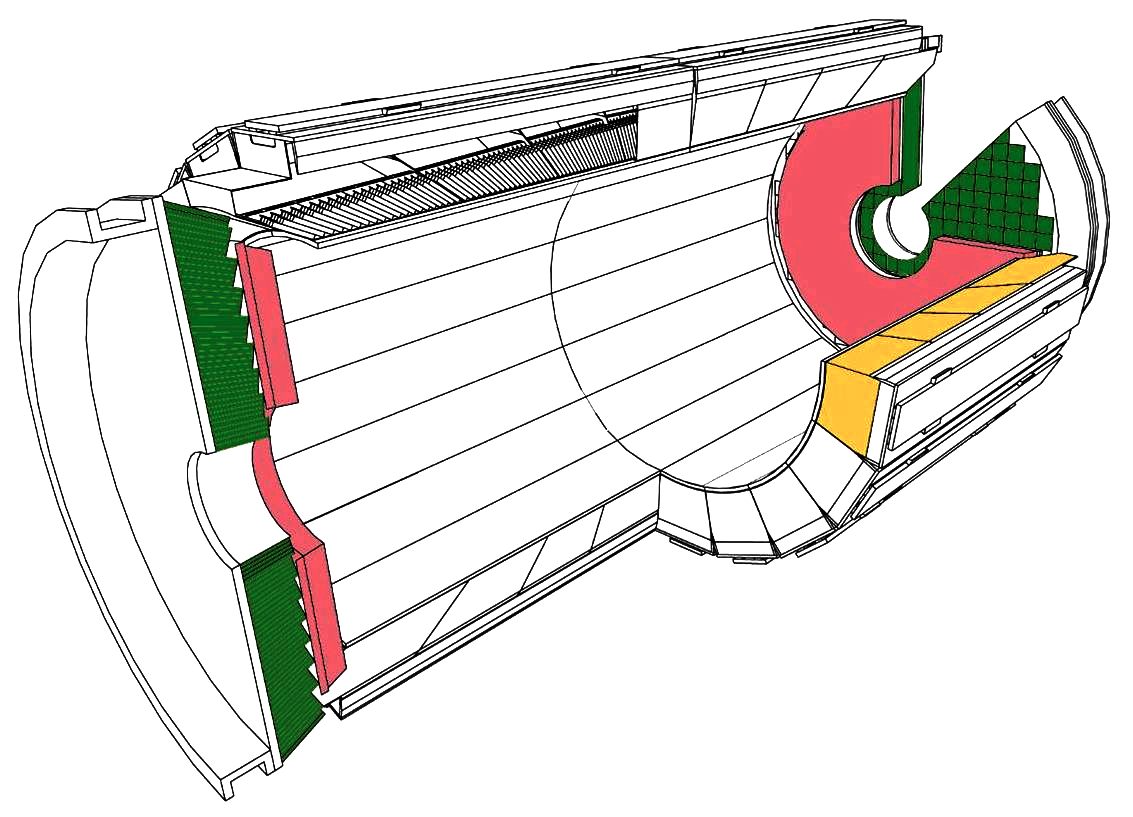
\includegraphics[width=0.7\textwidth]{figures/cms/ecal.jpg}
    \caption{A schematic of the CMS electromagnetic calorimeter showing the barrel supermodules (yellow), the individual barrel crystals (black,top left), the endcap modules (green) and the pre-shower detectors (pink)~\cite{Chatrchyan:2008aa}.}
    \label{fig:cms:ecal}
\end{figure}

Having no longitudinal segmentation, the ECAL relies on an accurate reconstruction of the event primary vertex, provided by the tracker, in order to reconstruct the photon angle correctly.

The obtained energy resolution of the ECAL can be parametrized in three parts: a stochastic, a noise and a constant term~\cite{Adzic:2007mi}. It is given as

\begin{equation*}
  \frac{\sigma \textrm{E}}{\textrm{E}} = \frac{2.8 \%}{\sqrt{\textrm{E}}}\oplus\frac{0.128 \GeV}{\textrm{E}}\oplus 0.3 \%
\end{equation*}

where the constant values were estimated in an electron test beam. The constant term of $0.3 \%$ is dominated by the non-uniformity in longitudinal light collection~\cite{1742-6596-587-1-012001}, and one of the main goals of the detector design was to get this term below 1\%. The energy resolution as a function of electron energy is shown in Figure~\ref{fig:cms:ecal-res}.

\begin{figure}[h] 
    \centering
    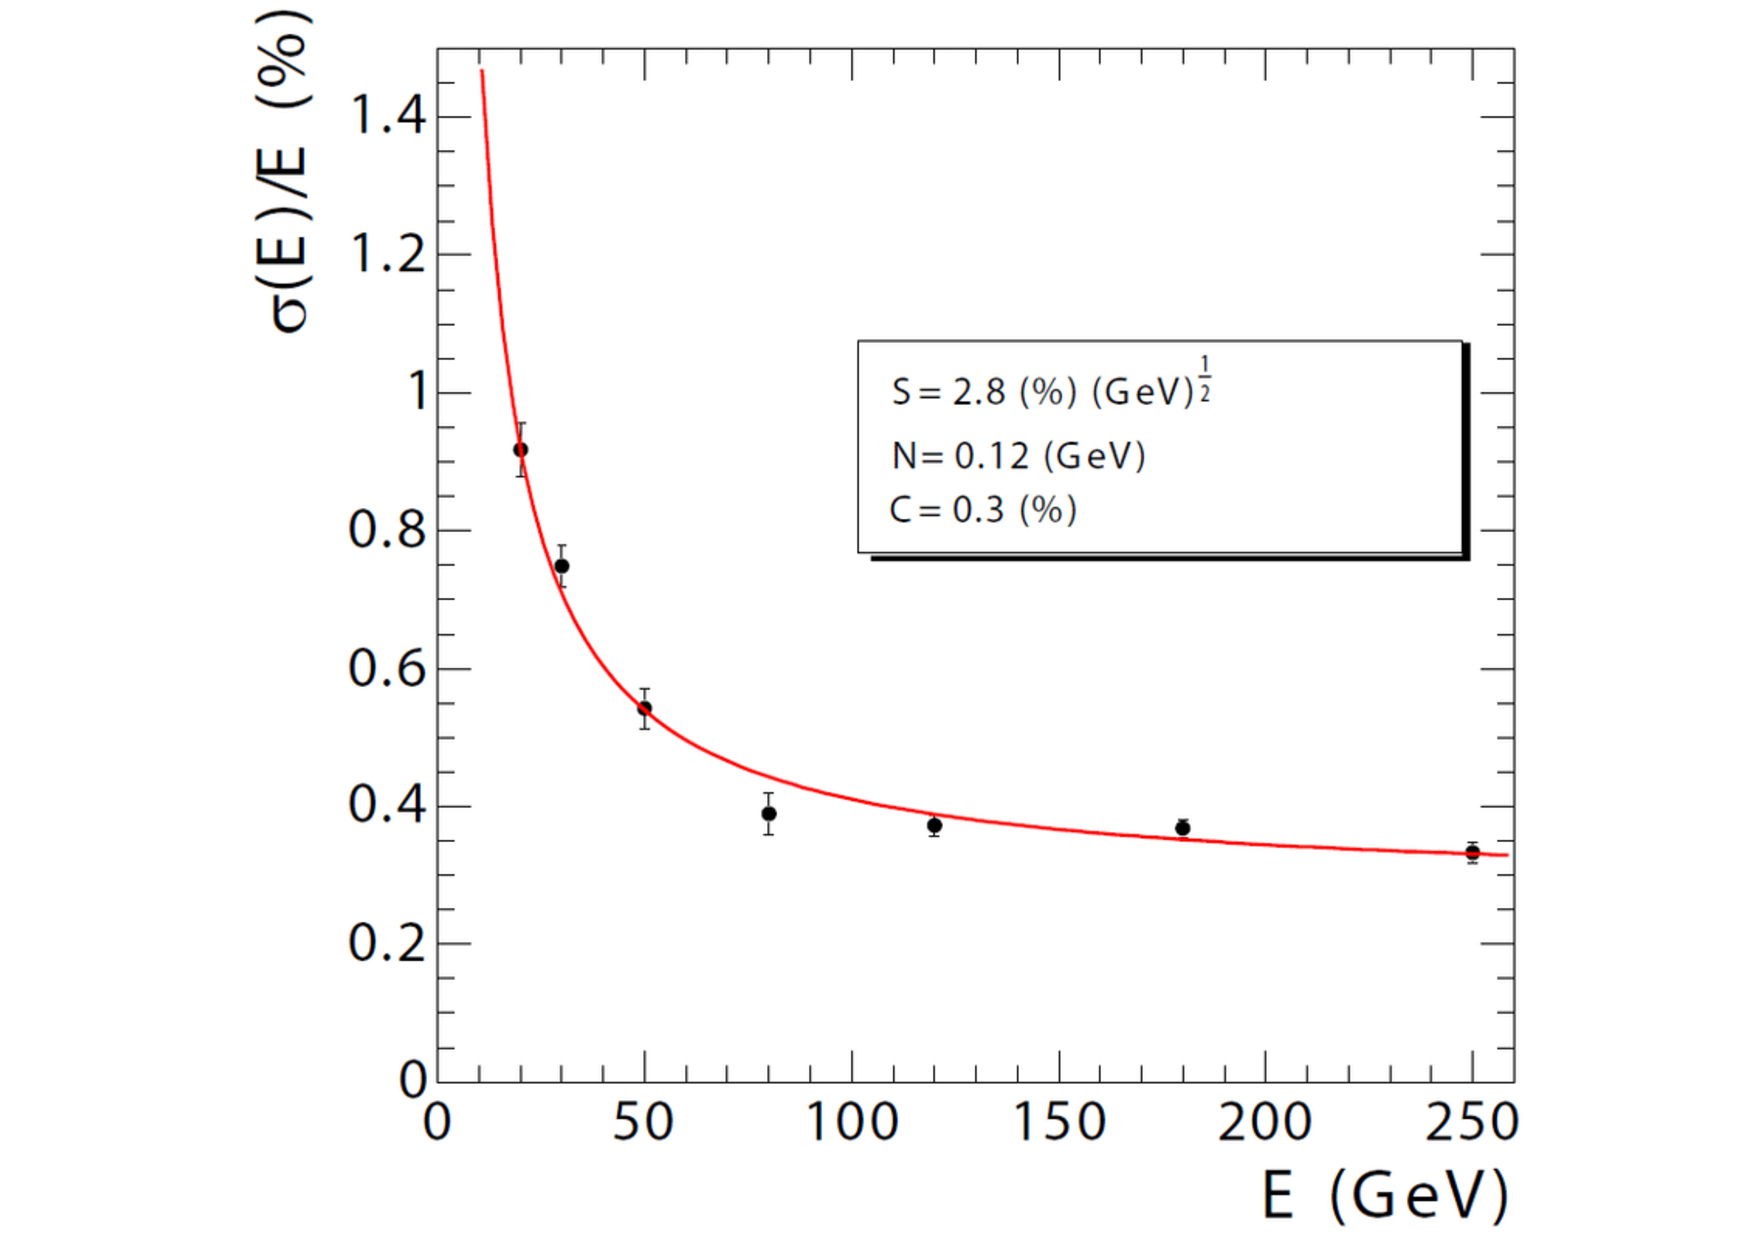
\includegraphics[width=0.6\textwidth]{figures/cms/ECAL-energy-resolution.pdf}
    \caption{The ECAL energy resolution as a function of electron energy as measured in an electron test beam.~\cite{Adzic:2007mi}}
    \label{fig:cms:ecal-res}
\end{figure}


\subsection{Hadron calorimeter}
Outside the crystal calorimeter is the hadron calorimeter (HCAL). It is the combined response of the ECAL and the HCAL that are responsible for measuring the energy of quarks, gluons and neutrinos through the reconstruction of particle jet energy and missing transverse energy. 
The HCAL is a sampling calorimeter, meaning it consists of alternating layers of dense brass absorber material and plastic scintillators. When a particle hits an absorber plate, it interacts with the absorber material and generates a shower of secondary particles which themselves generate new particle showers. These particles then generate light in the scintillating material which is proportional to their energy, and summing up the total amount of generated light over consecutive layers within a region, called a "tower", is representative of the initial particles energy.
The hadron calorimeter is split into four regions: the inner (HB) and outer (HO) barrel, the endcap (HE) and the forward region (HF).
A schematic of the CMS HCAL is shown in Figure~\ref{fig:cms:hcal}.

\begin{figure}[h] 
    \centering
    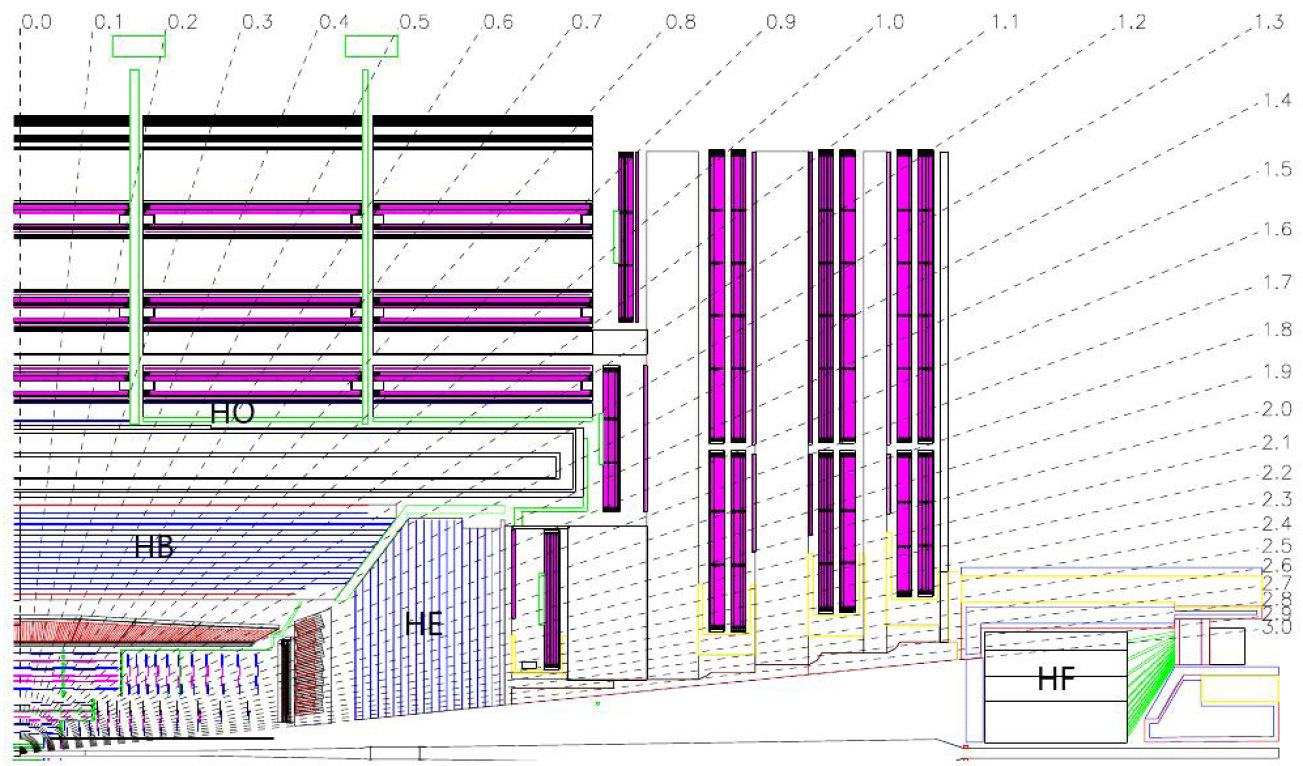
\includegraphics[width=0.6\textwidth]{figures/cms/HCAL.png}
    \caption{The four regions of the CMS hadron calorimeter:  the inner (HB) and outer (HO) barrel, the endcap (HE) and the forward region (HF)~\cite{Chatrchyan:2008aa}}
    \label{fig:cms:hcal}
\end{figure}

The inner barrel lies within the superconducting solenoid volume and covers the pseudorapidity range $|\eta|<1.3$.
It consists of 36 identical wedges, each of which weighing 26 tonnes, split into two half barrels (HB+ and HB-).
A photograph of the wedges taken during installation is shown in Figure~\ref{fig:cms:hcal-wedges}. 

\begin{figure}[h] 
    \centering
    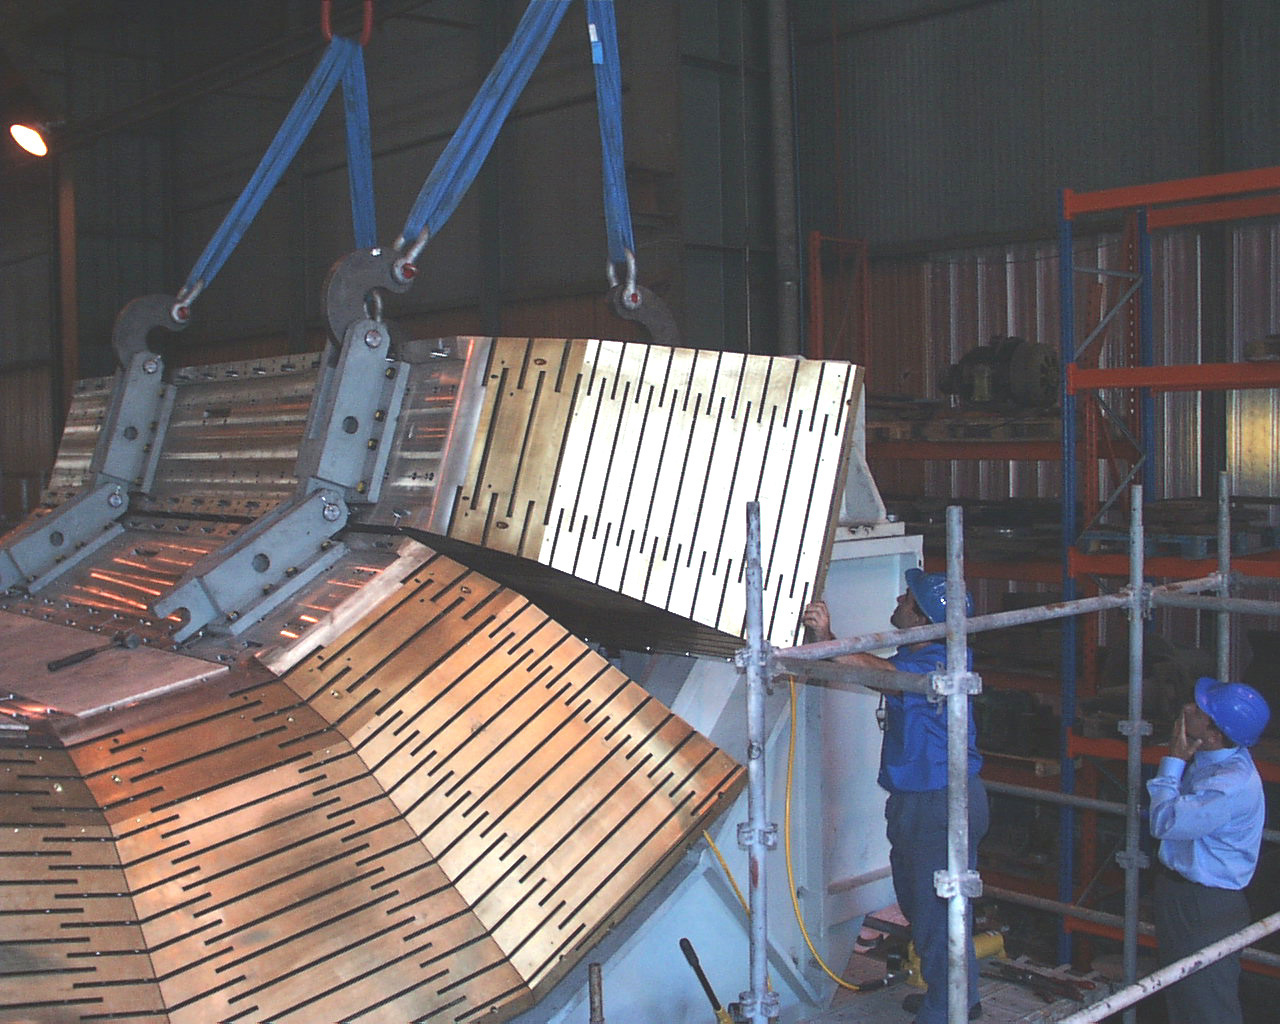
\includegraphics[width=0.6\textwidth]{figures/cms/hcal-2000-010_02.jpg}
    \caption{The installation of the barrel HCAL wedges consisting of alternating layers of brass absorber plates and plastic scintillator, each weighing roughly 26 tonnes~\cite{Veillet:41645}.}
    \label{fig:cms:hcal-wedges}
\end{figure}

The wedges are made up of flat brass absorber plates oriented parallel to the beam axis. These plates consist of a 4 \cm thick front steel plate followed by eight 5 \cm thick brass plates, six 5.6 \cm thick brass plates and ending with a 7.5 \cm thick steel back plate. The absorber plates are then alternated by 4 mm thick plastic scintillator tiles, the detectors active medium, which are read out using wavelength-shifting plastic fibers. The effective thickness of the barrel hadron calorimeter in terms of interaction lengths increases with the polar angle $\theta$, starting out at about 5.8 $\lambda_I$ at an angle of 90 degrees, and increases to 10.6 $\lambda_I$ at $|\eta|<1.3$.
As the energy resolution of the calorimeter depends on how much of the particles shower can be absorbed by the calorimeter, the quality of the energy measurement depends on its thickness. Due to the CMS design, the HB is confined to the volume between the ECAL (ending at a radius of 1.77 m) and the magnetic coil (starting at a radius of 2.95 m).
In the central $\eta$ region, the combined ECAL and HCAL interaction length is too small to sufficiently contain hadron showers. 
In order to ensure adequate sampling, especially of late starting showers, an additionally layer of scintillator has therefore been added outside of the solenoid coil. This is the outer barrel (HO). It uses the coil itself as absorbing material and increases the total barrel calorimeter interaction length to 11.8 $\lambda_I$.
The hadron calorimeter endcaps (HE) are located in the forward region close to the beam pipe and covers the pseudorapidity range $1.3 < |\eta|< 3.0$, a region containing about 35 \% of the particles produced in collisions. Due to its close proximity to the beam pipe, the endcaps need to handle extremely high rates as well as have a high radiation tolerance.
As the resolution in the endcap region anyways is limited by pile-up and magnetic field effects, the hadron calorimeter endcaps were designed to minimize the cracks between HB and HE rather than having the best single-particle resolution (as is the case for the barrel).
The absorber plates in the endcaps are mounted in a staggered geometry rather than on top of each other as is done in the barrel, in order to contain no dead material and provide a hermetic self-supporting construction.
In the very forward region, to achieve the most hermetic calorimeter possible, you find the hadron forward calorimeter (HF).
Stretching out to a pseudorapidity of $|\eta|= 5.2$, this detector is located so close to the beam pipe that the particle rate exceeds 10

\subsection{Muon chambers}
\section{Trigger system: From collision to disk}
